\documentclass[11pt,a4paper]{report}
\usepackage[textwidth=37em,vmargin=30mm]{geometry}
\usepackage{calc,xunicode,amsmath,amssymb,paralist,enumitem,tabu,booktabs,datetime2,xeCJK,xeCJKfntef,listings}
\usepackage{tocloft,fancyhdr,tcolorbox,xcolor,graphicx,eso-pic,xltxtra,xelatexemoji}

\newcommand{\envyear}[0]{2025}
\newcommand{\envdatestr}[0]{2025-01-17}
\newcommand{\envfinaldir}[0]{webdb/2025/20250117/final}

\usepackage[hidelinks]{hyperref}
\hypersetup{
    colorlinks=false,
    pdfpagemode=FullScreen,
    pdftitle={Web Digest - \envdatestr}
}

\setlength{\cftbeforechapskip}{10pt}
\renewcommand{\cftchapfont}{\rmfamily\bfseries\large\raggedright}
\setlength{\cftbeforesecskip}{2pt}
\renewcommand{\cftsecfont}{\sffamily\small\raggedright}

\setdefaultleftmargin{2em}{2em}{1em}{1em}{1em}{1em}

\usepackage{xeCJK,xeCJKfntef}
\xeCJKsetup{PunctStyle=plain,RubberPunctSkip=false,CJKglue=\strut\hskip 0pt plus 0.1em minus 0.05em,CJKecglue=\strut\hskip 0.22em plus 0.2em}
\XeTeXlinebreaklocale "zh"
\XeTeXlinebreakskip = 0pt


\setmainfont{Brygada 1918}
\setromanfont{Brygada 1918}
\setsansfont{IBM Plex Sans}
\setmonofont{JetBrains Mono NL}
\setCJKmainfont{Noto Serif CJK SC}
\setCJKromanfont{Noto Serif CJK SC}
\setCJKsansfont{Noto Sans CJK SC}
\setCJKmonofont{Noto Sans CJK SC}

\setlength{\parindent}{0pt}
\setlength{\parskip}{8pt}
\linespread{1.15}

\lstset{
	basicstyle=\ttfamily\footnotesize,
	numbersep=5pt,
	backgroundcolor=\color{black!5},
	showspaces=false,
	showstringspaces=false,
	showtabs=false,
	tabsize=2,
	captionpos=b,
	breaklines=true,
	breakatwhitespace=true,
	breakautoindent=true,
	linewidth=\textwidth
}






\newcommand{\coverpic}[2]{
    % argv: itemurl, authorname
    Cover photo by #2~~(\href{#1}{#1})
}
\newcommand{\makeheader}[0]{
    \begin{titlepage}
        % \newgeometry{hmargin=15mm,tmargin=21mm,bmargin=12mm}
        \begin{center}
            
            \rmfamily\scshape
            \fontspec{BaskervilleF}
            \fontspec{Old Standard}
            \fontsize{59pt}{70pt}\selectfont
            WEB\hfill DIGEST
            
            \vfill
            % \vskip 30pt
            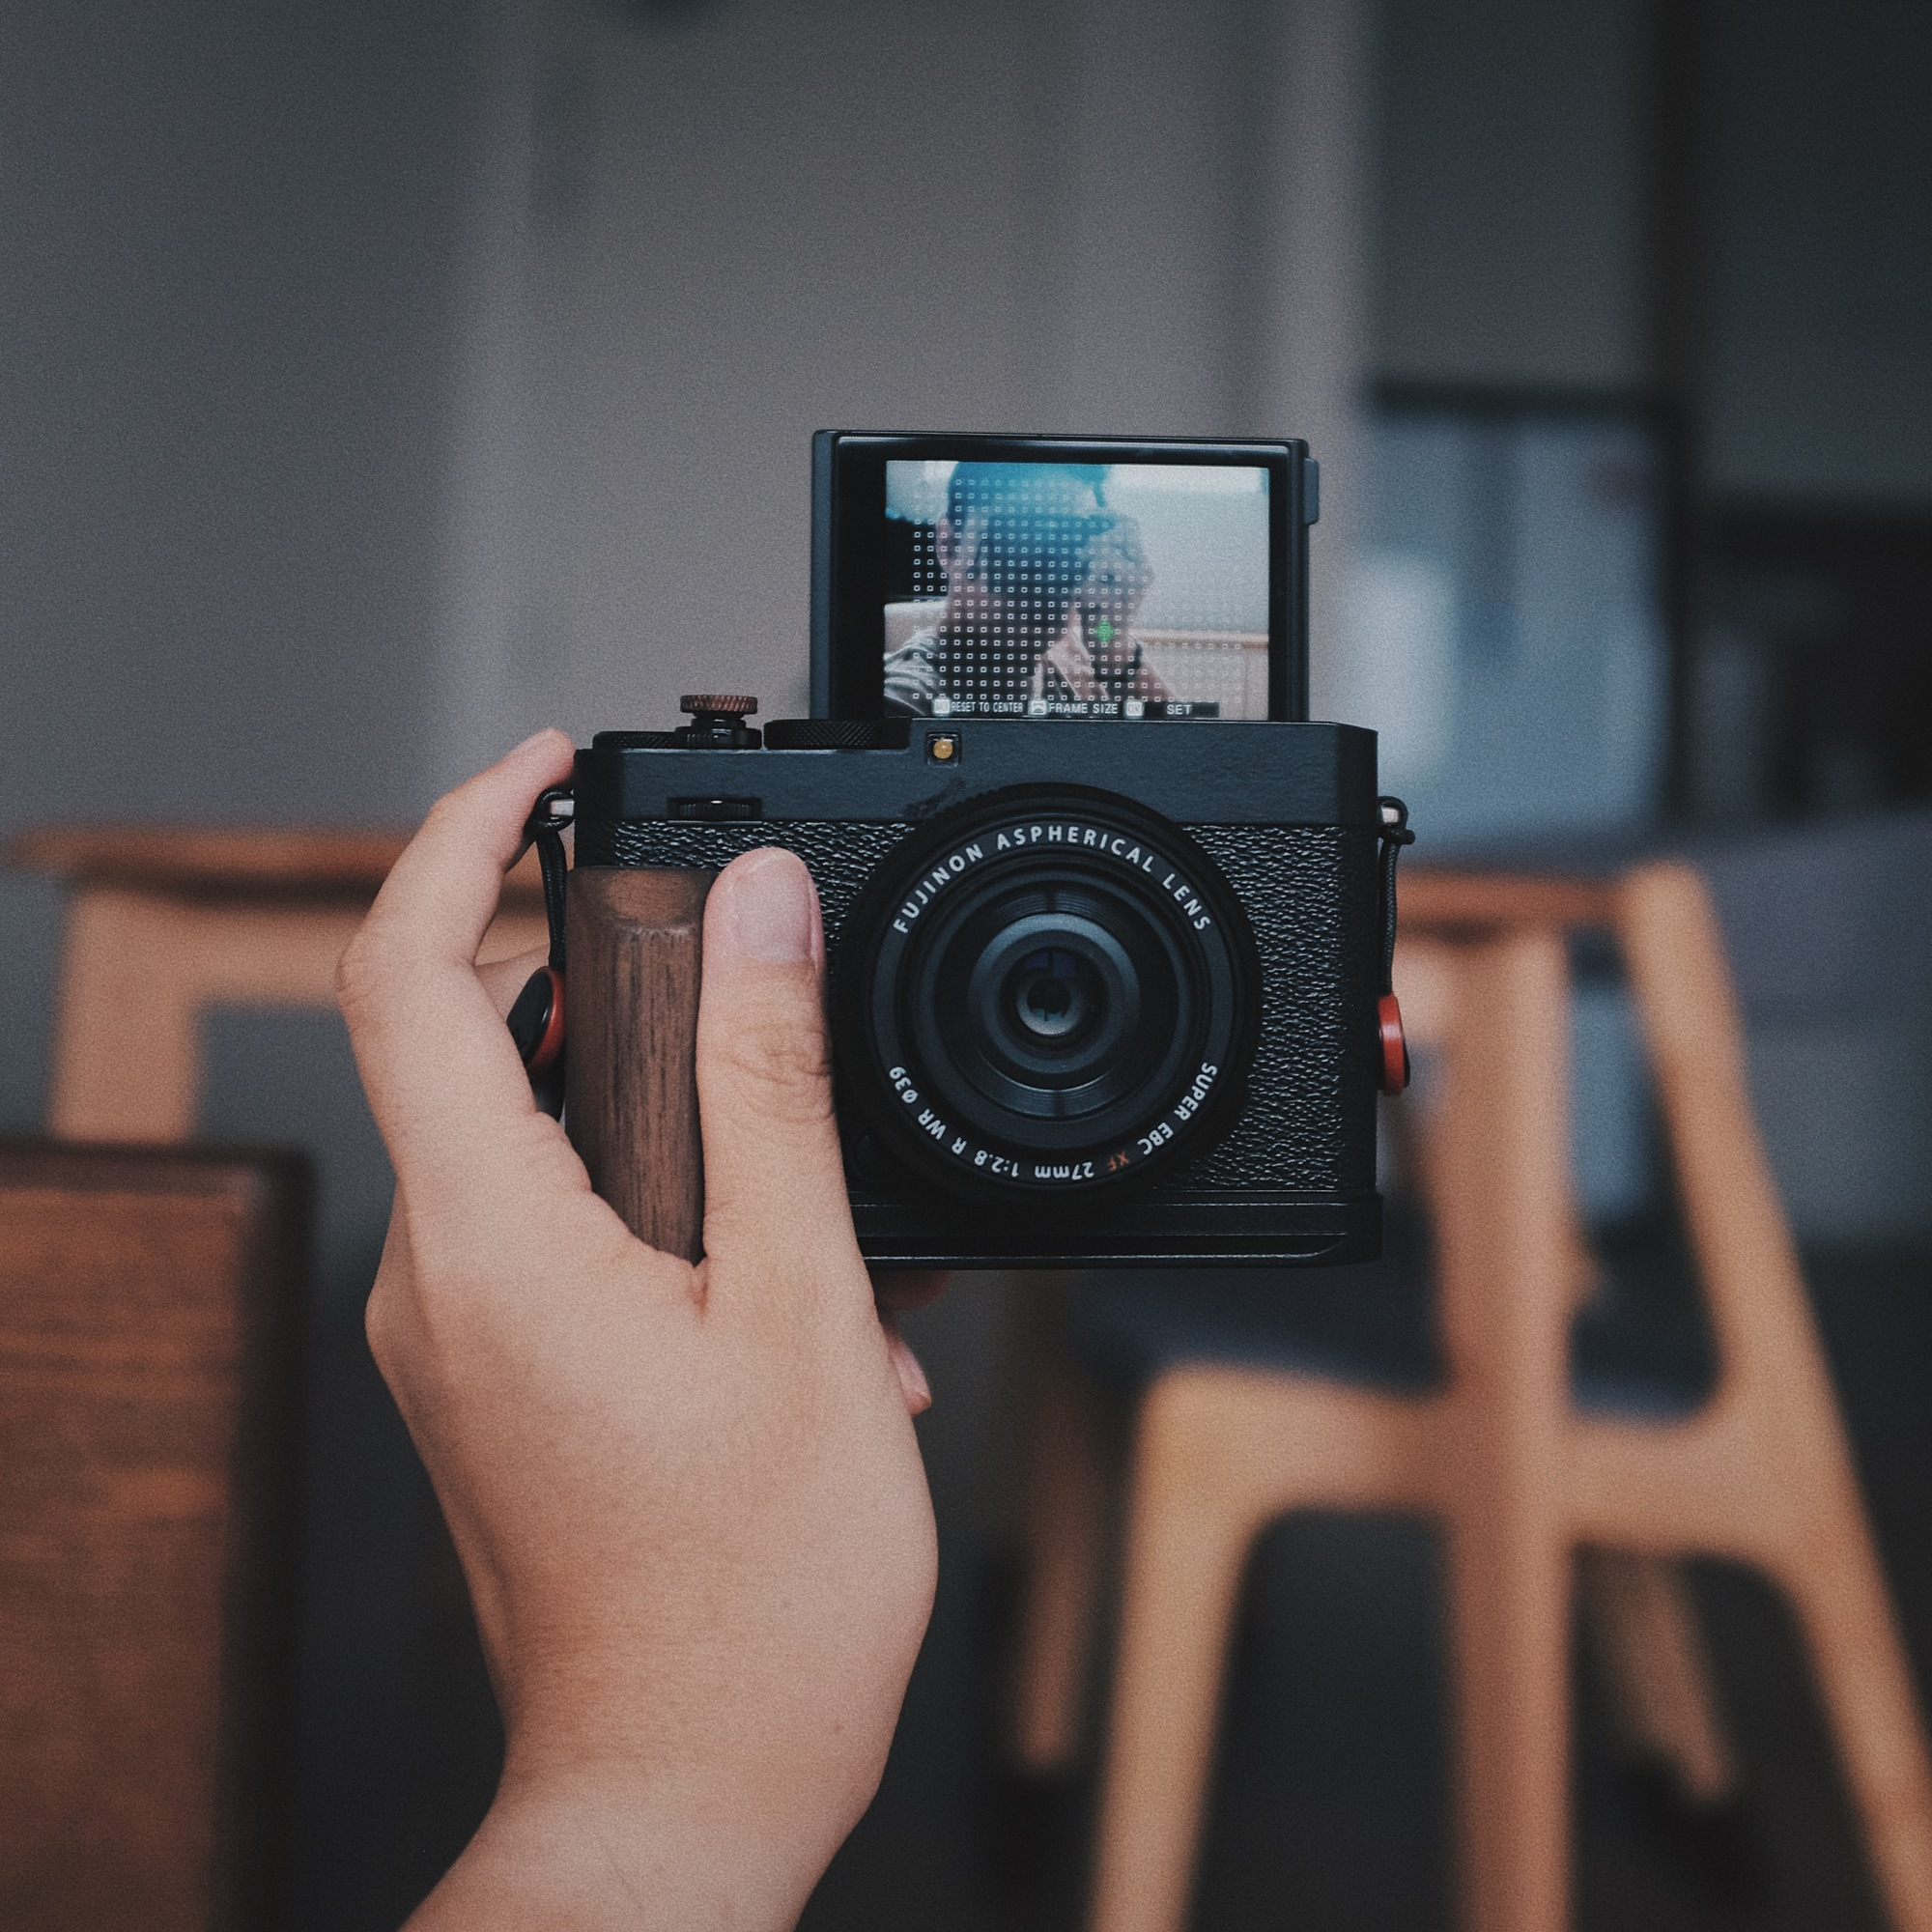
\includegraphics[width=\linewidth]{\envfinaldir/coverpic-prod.jpg}\par
            % \vskip 30pt
            \vfill

            \normalsize\rmfamily\scshape
            \copyright{} The Web Digest Project \hfill\large \envdatestr
        \end{center}
    \end{titlepage}
    % \restoregeometry
}
\newcommand{\simplehref}[1]{%
    \textcolor{blue!80!green}{\href{#1}{#1}}%
}
\renewcommand{\contentsname}{\center\Huge\sffamily\bfseries Contents\par\vskip 20pt}
\newcounter{ipartcounter}
\setcounter{ipartcounter}{0}
\newcommand{\ipart}[1]{
    % \vskip 20pt
    \clearpage
    \stepcounter{ipartcounter}
    \phantomsection
    \addcontentsline{toc}{chapter}{#1}
    % \begin{center}
    %     \Huge
    %     \sffamily\bfseries
    %     #1
    % \end{center}
    % \vskip 20pt plus 7pt
}
\newcounter{ichaptercounter}
\setcounter{ichaptercounter}{0}
\newcommand{\ichapter}[1]{
    % \vskip 20pt
    \clearpage
    \stepcounter{ichaptercounter}
    \phantomsection
    \addcontentsline{toc}{section}{\numberline{\arabic{ichaptercounter}}#1}
    \begin{center}
        \Huge
        \sffamily\bfseries
        #1
    \end{center}
    \vskip 20pt plus 7pt
}
\newcommand{\entrytitlefont}[1]{\subsection*{\raggedright\Large\sffamily\bfseries#1}}
\newcommand{\entryitemGeneric}[2]{
    % argv: title, url
    \parbox{\linewidth}{
        \entrytitlefont{#1}\par\vskip 5pt
        \footnotesize\ttfamily\mdseries
        \simplehref{#2}
    }\vskip 11pt plus 11pt minus 1pt
}
\newcommand{\entryitemGithub}[3]{
    % argv: title, url, desc
    \parbox{\linewidth}{
        \entrytitlefont{#1}\par\vskip 5pt
        \footnotesize\ttfamily\mdseries
        \simplehref{#2}\par\vskip 5pt
        \small\rmfamily\mdseries#3
    }\vskip 11pt plus 11pt minus 1pt
}
\newcommand{\entryitemAp}[3]{
    % argv: title, url, desc
    \parbox{\linewidth}{
        \entrytitlefont{#1}\par\vskip 5pt
        \footnotesize\ttfamily\mdseries
        \simplehref{#2}\par\vskip 5pt
        \small\rmfamily\mdseries#3
    }\vskip 11pt plus 11pt minus 1pt
}
\newcommand{\entryitemHackernews}[3]{
    % argv: title, hnurl, rawurl
    % \parbox{\linewidth}{
    %     \entrytitlefont{#1}\par\vskip 5pt
    %     \footnotesize\ttfamily\mdseries
    %     \simplehref{#3}\par
    %     \textcolor{black!50}{\href{#2}{#2}}
    % }\vskip 11pt plus 11pt minus 1pt
    \begin{minipage}{\linewidth}
            \entrytitlefont{#1}\par\vskip 5pt
            \footnotesize\ttfamily\mdseries
            \simplehref{#3}\par
            \textcolor{black!50}{\href{#2}{#2}}
    \end{minipage}\par\vskip 11pt plus 11pt minus 1pt
}







\begin{document}

\makeheader

\tableofcontents\clearpage




\ipart{Developers}
\ichapter{Hacker News}
\entryitemTwoLinks{Starship Flight 7}{https://news.ycombinator.com/item?id=42731091}{https://www.spacex.com/launches/mission/?missionId=starship-flight-7?submit}

\entryitemTwoLinks{Suchir Balaji Case Reopened: From `Suicide' to 'Active Investigation'}{https://news.ycombinator.com/item?id=42729677}{https://www.republicbiz.com/companies/suchir-balaji-case-reopened-from-suicide-to-active-investigation}

\entryitemTwoLinks{David Lynch, Twin Peaks and Muholland Drive director, dies aged 78}{https://news.ycombinator.com/item?id=42728967}{https://www.theguardian.com/film/2025/jan/16/david-lynch-twin-peaks-and-muholland-drive-director-dies-aged-78}

\entryitemTwoLinks{Oh Shit, Git?}{https://news.ycombinator.com/item?id=42728916}{https://ohshitgit.com/}

\entryitemTwoLinks{David Lynch has died}{https://news.ycombinator.com/item?id=42728862}{https://variety.com/2025/film/news/david-lynch-dead-director-blue-velvet-twin-peaks-1236276106/}

\entryitemTwoLinks{Comment on 2015 mRNA paper suggests data re-used in different contexts}{https://news.ycombinator.com/item?id=42728165}{https://pubpeer.com/publications/323E84675EB2E849C56097D73D55FD\#1}

\entryitemTwoLinks{GitHub Linux ARM64 hosted runners now available for free in public repositories}{https://news.ycombinator.com/item?id=42728015}{https://github.blog/changelog/2025-01-16-linux-arm64-hosted-runners-now-available-for-free-in-public-repositories-public-preview/}

\entryitemTwoLinks{Six day and IP address certificate options in 2025}{https://news.ycombinator.com/item?id=42726678}{https://letsencrypt.org/2025/01/16/6-day-and-ip-certs/}

\entryitemTwoLinks{Test-driven development with an LLM for fun and profit}{https://news.ycombinator.com/item?id=42726584}{https://blog.yfzhou.fyi/posts/tdd-llm/}

\entryitemTwoLinks{Red Hat Woos VMware Shops with OpenShift Virtualization Engine}{https://news.ycombinator.com/item?id=42725862}{https://www.nextplatform.com/2025/01/15/red-hat-woos-vmware-shops-with-openshift-virtualization-engine/}

\entryitemTwoLinks{No Calls}{https://news.ycombinator.com/item?id=42725385}{https://keygen.sh/blog/no-calls/}

\entryitemTwoLinks{Nepenthes is a tarpit to catch AI web crawlers}{https://news.ycombinator.com/item?id=42725147}{https://zadzmo.org/code/nepenthes/}

\entryitemTwoLinks{No Billionares at FOSDEM}{https://news.ycombinator.com/item?id=42725057}{https://drewdevault.com/2025/01/16/2025-01-16-No-Billionares-at-FOSDEM-please.html}

\entryitemTwoLinks{Nintendo Switch 2}{https://news.ycombinator.com/item?id=42724823}{https://www.nintendo.com/successor/en-gb/index.html}

\entryitemTwoLinks{Nokia's internal presentation after iPhone was launched (2007) [pdf]}{https://news.ycombinator.com/item?id=42724761}{https://nokia-apple-iphone-was-launched-presentation.tiiny.site/}

\entryitemTwoLinks{Show HN: I made an open source directory of where to showoff your projects}{https://news.ycombinator.com/item?id=42724757}{https://github.com/KingMenes/awesome-launch}

\entryitemTwoLinks{Nintendo announces the Switch 2 [video]}{https://news.ycombinator.com/item?id=42724621}{https://www.youtube.com/watch?v=itpcsQQvgAQ}

\entryitemTwoLinks{I ditched the algorithm for RSS}{https://news.ycombinator.com/item?id=42724284}{https://joeyehand.com/blog/2025/01/15/i-ditched-the-algorithm-for-rssand-you-should-too/}

\entryitemTwoLinks{Apple interoperability efforts under EU law falls short, advocacy groups argue}{https://news.ycombinator.com/item?id=42723504}{https://www.theregister.com/2025/01/16/apple\_dma\_compliance\_criticized/}

\entryitemTwoLinks{Mathematicians discover new way for spheres to 'kiss'}{https://news.ycombinator.com/item?id=42723406}{https://www.quantamagazine.org/mathematicians-discover-new-way-for-spheres-to-kiss-20250115/}\ichapter{Phoronix}
\entryitemGeneric{\hskip 0pt{}The Most Exciting Kernel Optimizations, New Hardware Support \& Other Linux 6.13 Features}{https://www.phoronix.com/news/Linux-6.13-Features-Reminder}

\entryitemGeneric{\hskip 0pt{}Intel Arc B570 Graphics Performance On Linux}{https://www.phoronix.com/review/intel-arc-b570-linux}

\entryitemGeneric{\hskip 0pt{}AMDGPU VirtIO Native Context Merged: Native AMD Driver Support Within Guest VMs}{https://www.phoronix.com/news/AMDGPU-VirtIO-Native-Mesa-25.0}

\entryitemGeneric{\hskip 0pt{}Fedora KDE Plasma Edition Aims To Appeal To Multimedia Enthusiasts \& Content Creators}{https://www.phoronix.com/news/Fedora-KDE-Edition-Plan}

\entryitemGeneric{\hskip 0pt{}AT\_EXECVE\_CHECK Submitted For Linux 6.14 To Help With Consistent Security}{https://www.phoronix.com/news/Linux-6.14-AT\_EXECVE\_CHECK}

\entryitemGeneric{\hskip 0pt{}CXL Address Translation Support For AMD Zen 5 Sees Linux Patches}{https://www.phoronix.com/news/AMD-Zen5-CXL-Translation-v1}

\entryitemGeneric{\hskip 0pt{}Expanding Web Camera Support Among Newer Intel Laptops Planned For Fedora 42}{https://www.phoronix.com/news/Intel-More-Webcams-Fedora-42}

\entryitemGeneric{\hskip 0pt{}GCC Goes Ahead With The ARM64 ILP32 Deprecation}{https://www.phoronix.com/news/GCC-Deprecates-ARM64-ILP32}

\entryitemGeneric{\hskip 0pt{}Fedora 42 Is Looking At Switching To EROFS For Its Live Media}{https://www.phoronix.com/news/Fedora-42-Considers-EROFS}\ichapter{Dribbble}
\entryitemGeneric{\hskip 0pt{}Wine Label}{https://dribbble.com/shots/25485370-Wine-Label}

\entryitemGeneric{\hskip 0pt{}Puzzle Fintech Website Design}{https://dribbble.com/shots/25394559-Puzzle-Fintech-Website-Design}

\entryitemGeneric{\hskip 0pt{}RoundRobin 2.0}{https://dribbble.com/shots/25479558-RoundRobin-2-0}

\entryitemGeneric{\hskip 0pt{}Pemberton's Formula}{https://dribbble.com/shots/25480158-Pemberton-s-Formula}

\entryitemGeneric{\hskip 0pt{}Black Cats}{https://dribbble.com/shots/25478711-Black-Cats}

\entryitemGeneric{\hskip 0pt{}N\&R Social Media}{https://dribbble.com/shots/25159226-N-R-Social-Media}

\entryitemGeneric{\hskip 0pt{}Vertical Logos from the Portfolio}{https://dribbble.com/shots/25479968-Vertical-Logos-from-the-Portfolio}

\entryitemGeneric{\hskip 0pt{}Top 9 logos of 2024}{https://dribbble.com/shots/25479840-Top-9-logos-of-2024}

\entryitemGeneric{\hskip 0pt{}Developing new skills}{https://dribbble.com/shots/25479409-Developing-new-skills}

\entryitemGeneric{\hskip 0pt{}Gillespie Farms™}{https://dribbble.com/shots/25474556-Gillespie-Farms}

\entryitemGeneric{\hskip 0pt{}Faith Education Icons}{https://dribbble.com/shots/25422138-Faith-Education-Icons}

\entryitemGeneric{\hskip 0pt{}Round Robin}{https://dribbble.com/shots/25467606-Round-Robin}

\entryitemGeneric{\hskip 0pt{}Nexos crypto wallet}{https://dribbble.com/shots/25464532-Nexos-crypto-wallet}

\entryitemGeneric{\hskip 0pt{}Kraken Illustration}{https://dribbble.com/shots/25468020-Kraken-Illustration}

\entryitemGeneric{\hskip 0pt{}B}{https://dribbble.com/shots/25466481-B}

\entryitemGeneric{\hskip 0pt{}Document Scanner App}{https://dribbble.com/shots/25466972-Document-Scanner-App}

\entryitemGeneric{\hskip 0pt{}The best route to the corner office}{https://dribbble.com/shots/25468475-The-best-route-to-the-corner-office}

\entryitemGeneric{\hskip 0pt{}Pythagoras}{https://dribbble.com/shots/25467709-Pythagoras}

\entryitemGeneric{\hskip 0pt{}Learning App Design}{https://dribbble.com/shots/25458950-Learning-App-Design}

\entryitemGeneric{\hskip 0pt{}Cub Studio Process}{https://dribbble.com/shots/25456521-Cub-Studio-Process}

\entryitemGeneric{\hskip 0pt{}Southland Provisions}{https://dribbble.com/shots/25456279-Southland-Provisions}

\entryitemGeneric{\hskip 0pt{}Polar Bear + Baby (2012)}{https://dribbble.com/shots/25454483-Polar-Bear-Baby-2012}

\entryitemGeneric{\hskip 0pt{}SHOWREEL 24'}{https://dribbble.com/shots/25450148-SHOWREEL-24}

\entryitemGeneric{\hskip 0pt{}Yacht Life}{https://dribbble.com/shots/25456479-Yacht-Life}


\ipart{Developers~~~~(zh-Hans)}
\ichapter{Solidot}
\entryitemGeneric{\hskip 0pt{}RISC-V 开发商算能公司被美国列入实体名单}{https://www.solidot.org/story?sid=80353}

\entryitemGeneric{\hskip 0pt{}Blue Origin 的重型火箭 New Glenn 首次抵达轨道}{https://www.solidot.org/story?sid=80352}

\entryitemGeneric{\hskip 0pt{}Proton CEO 拥抱特朗普引发争议}{https://www.solidot.org/story?sid=80351}

\entryitemGeneric{\hskip 0pt{}动视对微软 Xbox Game Pass 订阅量增加帮助不大}{https://www.solidot.org/story?sid=80350}

\entryitemGeneric{\hskip 0pt{}日英意下一代战斗机计划本年内开始制造试制机}{https://www.solidot.org/story?sid=80349}

\entryitemGeneric{\hskip 0pt{}新泽西州州长呼吁 K-12 学校禁止学生使用手机}{https://www.solidot.org/story?sid=80348}

\entryitemGeneric{\hskip 0pt{}英特尔开源 Tofino P4 软件}{https://www.solidot.org/story?sid=80347}

\entryitemGeneric{\hskip 0pt{}LinkedIn 用 AI 劝阻求职者不要申请不符合条件的职位}{https://www.solidot.org/story?sid=80346}

\entryitemGeneric{\hskip 0pt{}深圳大疆让无人机操作人员决定是否在禁飞区飞行}{https://www.solidot.org/story?sid=80345}

\entryitemGeneric{\hskip 0pt{}Telegram 关闭 Z-Library 和 Anna's Archive 频道}{https://www.solidot.org/story?sid=80344}

\entryitemGeneric{\hskip 0pt{}是时候重新定义肥胖}{https://www.solidot.org/story?sid=80343}

\entryitemGeneric{\hskip 0pt{}太长时间的自控会增加类睡眠大脑活动}{https://www.solidot.org/story?sid=80342}

\entryitemGeneric{\hskip 0pt{}用 AI 将电子书转变成有声书}{https://www.solidot.org/story?sid=80341}

\entryitemGeneric{\hskip 0pt{}GOG 加入欧洲游戏保存组织 }{https://www.solidot.org/story?sid=80340}

\entryitemGeneric{\hskip 0pt{}TikTok 计划周日关闭其美国服务}{https://www.solidot.org/story?sid=80339}

\entryitemGeneric{\hskip 0pt{}丰田连续五年新车销量第一}{https://www.solidot.org/story?sid=80338}

\entryitemGeneric{\hskip 0pt{}沉迷长寿的科技富豪停服可能加速衰老的长寿药}{https://www.solidot.org/story?sid=80337}

\entryitemGeneric{\hskip 0pt{}微软 1 月例行更新修复 161 个漏洞}{https://www.solidot.org/story?sid=80336}

\entryitemGeneric{\hskip 0pt{}Meta 根据绩效裁员 3600 人}{https://www.solidot.org/story?sid=80335}

\entryitemGeneric{\hskip 0pt{}美国预测到 2033 年死亡人口将超过出生人口}{https://www.solidot.org/story?sid=80334}\ichapter{V2EX}
\entryitemGeneric{\hskip 0pt{}[程序员] 支付宝这次的 Bug 有点严重啊}{https://www.v2ex.com/t/1105707}

\entryitemGeneric{\hskip 0pt{}[日本] 现在日本有什么好买的?}{https://www.v2ex.com/t/1105706}

\entryitemGeneric{\hskip 0pt{}[macOS] macOS 15.2 无法拨打电话,拨打时会变成启动浏览器,并没有打开什么网页。但上个版本可以正常拨打。}{https://www.v2ex.com/t/1105705}

\entryitemGeneric{\hskip 0pt{}[电影] David Lynch 去世}{https://www.v2ex.com/t/1105704}

\entryitemGeneric{\hskip 0pt{}[分享发现] (支付宝事故后续)承诺不会向用户追款}{https://www.v2ex.com/t/1105703}

\entryitemGeneric{\hskip 0pt{}[分享创造] 不是程序员又利用 ai 生成一个工具型网站,这次还使用了 Next.js 框架}{https://www.v2ex.com/t/1105702}

\entryitemGeneric{\hskip 0pt{}[生活] 2024: 离开上海并在东京转职到 Woven by Toyota 写 Rust}{https://www.v2ex.com/t/1105701}

\entryitemGeneric{\hskip 0pt{}[OpenAI] 现在网页端是不是不降智了?}{https://www.v2ex.com/t/1105700}

\entryitemGeneric{\hskip 0pt{}[VPS] VPS 上套了 Cloudflare warp,速度狂慢,最有可能的状况是什么?}{https://www.v2ex.com/t/1105699}

\entryitemGeneric{\hskip 0pt{}[macOS] MacBook 网络连接有点断断续续的,请问有哪些排查的工具}{https://www.v2ex.com/t/1105697}

\entryitemGeneric{\hskip 0pt{}[奇思妙想] 分享一下 Talkatone 注册和转移到 Google Voice 的过程}{https://www.v2ex.com/t/1105696}

\entryitemGeneric{\hskip 0pt{}[上海] 上海周末两天哪里好玩?}{https://www.v2ex.com/t/1105693}

\entryitemGeneric{\hskip 0pt{}[PlayStation 5] ps portal 如何连 WiFi 不用加速器}{https://www.v2ex.com/t/1105692}

\entryitemGeneric{\hskip 0pt{}[分享创造] 做了一个 2024 年度独立博客年终总结随机浏览网站——发现他人的精彩,找到自己的方向}{https://www.v2ex.com/t/1105691}

\entryitemGeneric{\hskip 0pt{}[游戏开发] 类似 Duolingo 的应用,在国内上架移动端需要游戏版号吗}{https://www.v2ex.com/t/1105690}

\entryitemGeneric{\hskip 0pt{}[计算机] 求推荐笔记本,想问下现在哪些笔记本有类似旁路充电的功能}{https://www.v2ex.com/t/1105689}

\entryitemGeneric{\hskip 0pt{}[问与答] 请问大家有推荐的开源图床吗}{https://www.v2ex.com/t/1105688}

\entryitemGeneric{\hskip 0pt{}[酷工作] 海外售中迁移架构师}{https://www.v2ex.com/t/1105687}

\entryitemGeneric{\hskip 0pt{}[程序员] 大家会利用 Github Star 信息进行推广自己的开源项目吗?效果如何}{https://www.v2ex.com/t/1105685}

\entryitemGeneric{\hskip 0pt{}[问与答] 请教大佬,视频播放时,进行全屏,画面会短暂暂停,声音是始终连续播放, infuse 和 iina 都是这样}{https://www.v2ex.com/t/1105684}

\entryitemGeneric{\hskip 0pt{}[宽带症候群] 关于 tailscale 的一些疑问}{https://www.v2ex.com/t/1105682}

\entryitemGeneric{\hskip 0pt{}[生活] 用了一年多的 wise ,突然要地址证明}{https://www.v2ex.com/t/1105681}

\entryitemGeneric{\hskip 0pt{}[Elasticsearch] opensearch data 节点,分片数均匀,磁盘存储不均匀, CPU 有些很高有些很低}{https://www.v2ex.com/t/1105679}

\entryitemGeneric{\hskip 0pt{}[问与答] 驾照只能提前 90 天更新吗,春节回去想更新,但是还没到 90 天}{https://www.v2ex.com/t/1105678}

\entryitemGeneric{\hskip 0pt{}[Nintendo Switch] 任天堂发布 Switch 2 预告片,并宣布于 2025.4.2 展开直面会}{https://www.v2ex.com/t/1105677}

\entryitemGeneric{\hskip 0pt{}[游戏] 大家有没有让人上头的小游戏,简单而且让人上瘾}{https://www.v2ex.com/t/1105675}

\entryitemGeneric{\hskip 0pt{}[信息安全] 如果抽卡游戏用的不是密码学安全的随机数算法(我觉得大部分游戏都不是),是不是有可能从客户端控制服务器的随机抽卡结果?}{https://www.v2ex.com/t/1105674}

\entryitemGeneric{\hskip 0pt{}[推广] 倒数日 App,限时特惠,了解一下?}{https://www.v2ex.com/t/1105673}

\entryitemGeneric{\hskip 0pt{}[分享创造] EnglishDaily 一款免费的每日英语学习网站}{https://www.v2ex.com/t/1105672}

\entryitemGeneric{\hskip 0pt{}[生活] 拼多多竟然还有这种东西,建议在农村过年的买个玩玩,我先买为敬}{https://www.v2ex.com/t/1105670}

\entryitemGeneric{\hskip 0pt{}[分享创造] 英文文本翻转网站 https://upsidedowntext.vip}{https://www.v2ex.com/t/1105667}

\entryitemGeneric{\hskip 0pt{}[酷工作] 找一家可以远程的前端工作,本人技术栈 Vue3 系列}{https://www.v2ex.com/t/1105666}

\entryitemGeneric{\hskip 0pt{}[问与答] 2025 年了, Safari 下有手势拖拽插件吗}{https://www.v2ex.com/t/1105665}

\entryitemGeneric{\hskip 0pt{}[问与答] MacOS 窗口焦点 bug}{https://www.v2ex.com/t/1105664}

\entryitemGeneric{\hskip 0pt{}[YubiKey] YubiKey 5 NFC 两枚打包 咸鱼 750 出}{https://www.v2ex.com/t/1105662}

\entryitemGeneric{\hskip 0pt{}[问与答] 有多少人是 彩礼一分不留,还另外带嫁妆(钱)的?}{https://www.v2ex.com/t/1105661}

\entryitemGeneric{\hskip 0pt{}[Apple] 求推荐个 MacBook 用的无线或者蓝牙耳机}{https://www.v2ex.com/t/1105660}

\entryitemGeneric{\hskip 0pt{}[问与答] 工行追加贷有什么坑}{https://www.v2ex.com/t/1105658}

\entryitemGeneric{\hskip 0pt{}[问与答] 3599 的 Mac mini 4 丐版好像很容易买到?}{https://www.v2ex.com/t/1105657}

\entryitemGeneric{\hskip 0pt{}[问与答] 网格员们开始查房扰民了}{https://www.v2ex.com/t/1105656}

\entryitemGeneric{\hskip 0pt{}[问与答] 手机推荐}{https://www.v2ex.com/t/1105655}

\entryitemGeneric{\hskip 0pt{}[浏览器] 百分浏览器和 Catsxp 浏览器的同步功能是怎么实现的?}{https://www.v2ex.com/t/1105654}

\entryitemGeneric{\hskip 0pt{}[分享发现] 发现新出了一个设计页面的神器,我用它快速做了一个 RedNote 小红书博主精选页}{https://www.v2ex.com/t/1105652}

\entryitemGeneric{\hskip 0pt{}[问与答] 现在有跨平台的``灰鸽子''软件推荐嘛}{https://www.v2ex.com/t/1105651}

\entryitemGeneric{\hskip 0pt{}[信息安全] 关于 2FA 和密码}{https://www.v2ex.com/t/1105650}

\entryitemGeneric{\hskip 0pt{}[程序员] 谷歌浏览器可以实现有声自动播放视频吗}{https://www.v2ex.com/t/1105649}

\entryitemGeneric{\hskip 0pt{}[分享发现] 避雷 onedrive,纯低能应用}{https://www.v2ex.com/t/1105647}

\entryitemGeneric{\hskip 0pt{}[程序员] [付费咨询] NEPacketTunnelProvider}{https://www.v2ex.com/t/1105646}

\entryitemGeneric{\hskip 0pt{}[程序员] 公司被 docker 发律师函}{https://www.v2ex.com/t/1105645}

\entryitemGeneric{\hskip 0pt{}[淘宝] 香港开的银行卡.怎么可以在国内淘宝购物呢}{https://www.v2ex.com/t/1105644}


\ipart{Generic News}







\clearpage
\leavevmode\vfill
\footnotesize

Copyright \copyright{} 2023-2025 Neruthes and other contributors.

This document is published with CC BY-NC-ND 4.0 license.

The entries listed in this newsletter may be copyrighted by their respective creators.

This newsletter is generated by the Web Digest project.

The newsletters are also delivered via Telegram channel \CJKunderline{\href{https://t.me/webdigestchannel}{https://t.me/webdigestchannel}}.\\
RSS feed is available at \CJKunderline{\href{https://webdigest.pages.dev/rss.xml}{https://webdigest.pages.dev/rss.xml}}.

This newsletter is available in PDF at
\CJKunderline{\href{https://webdigest.pages.dev/}{https://webdigest.pages.dev/}}.

The source code being used to generate this newsletter is available at\\
\CJKunderline{\href{https://github.com/neruthes/webdigest}{https://github.com/neruthes/webdigest}}.

This newsletter is also available in
\CJKunderline{\href{http://webdigest.pages.dev/readhtml/\envyear/WebDigest-20250117.html}{HTML}} and
\CJKunderline{\href{https://github.com/neruthes/webdigest/blob/master/markdown/\envyear/WebDigest-20250117.md}{Markdown}}.


\coverpic{https://unsplash.com/photos/a-black-and-white-photo-of-a-bridge-qI2B4SPAji8}{Adam Hornyak}


\end{document}
